\label{sec:neuro_expl}

In this thesis the concepts specific to neuromorphic engineering will be used extensively. 
Before diving into the design and results of the proposed controllers, a clear understanding of these and other related concepts must be reached. 
Otherwise, comprehension of the choices or design decisions made will be difficult.

\section{Excitability}

The first step in the comprehension of neuronal system is the concept of excitability. In the words of \citet{excDef}, \enquote{Excitability is the property of a system to exhibit all-or-none response to pulse inputs}. 
In other words, the system exhibit nearly no response from pulses until the pulse amplitude crosses a certain threshold after which the system responds completely. 

In \cref{fig:excitability}, an example of an excitable behavior is displayed. 
As can be seen, a very small difference in the pulse amplitude resulted in a very different neuronal behavior. 
The lower pulse resulted in the output faithfully following the input while the output of the higher one exhibited a very different behavior with oscillation and  peaks far above the input. 
This specific behavior is known as bursting and will be discussed later.

\begin{figure}[htb]
    \centering
    \inserttikzfig{plots/excitability.tikz}
    \caption{Example of an excitable behavior. Generated using neuron model of \cref{sec:model}.}
    \label{fig:excitability}
\end{figure}

This kind of behavior is often seen in neuronal systems.
The all-or-none response is important to transform continuous input into discrete events. 
This discretization makes a system more resilient to noise and capable of reacting only when necessary.

This kind of response is desired in our controller since the effective control of the oscillation of a pendulum requires a very all-or-nothing control input. 
Indeed the moment of actuation is very important when controlling a pendulum and actuating at a bad time can lead to very poor results. 
Still, in  the words of \citet{excDef}, \enquote{\textins{Excitability} is instrumental in converting sensory signals into motor actions}.

To create an excitable system a localized positive feedback loop is necessary. 
Indeed, the switch between two different responses after the crossing of a threshold requires the activation of a positive feedback near the threshold. 
This feedback pushes the output of the system to generate the excitable event.

\section{Conductance-based neuron models}

Excitability being defined, neuronal models can be understood more clearly. Indeed, neurons are a prime example of an excitable system.

Basically, neurons are cells that are able to receive input from the external world, send messages to one another and send motor commands to muscles. 
Since a neuron can be relatively big, it is evident that its behavior may be different at different part of the cell. 
But, a common way to observe a neuron is to measure and model its activity in only one location.

As shown by \citet{neuronIons}, the state of a neurons at its axon membrane can be described by the flow of ionic currents. 
The magnitude of those current is determined by the potential across the interior and the exterior of the cell which opens or closed channels at a speed that is dependent on the channel type.
In turn these currents flowing into or out of the cell influence the potential across the interior and the exterior of the cell. 

This model is illustrated on \cref{fig:conductance_neuron}, where ionic currents are flowing through channels in the neuron membrane. Those channels activate and deactivate based on the membrane potential.

\begin{figure}[htb]
    \centering
    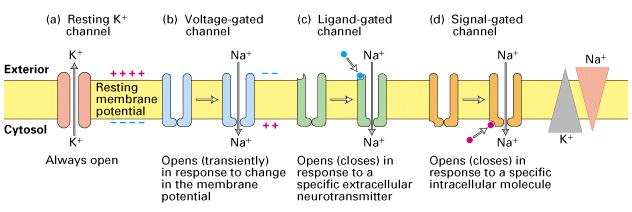
\includegraphics[width=.9\textwidth]{channels.png}
    \caption{Simplified diagram of a biological neuron membrane. (Diagram taken from \citet{channelDiagram})}
    \label{fig:conductance_neuron}
\end{figure}

\begin{figure}[htb]
    \centering
    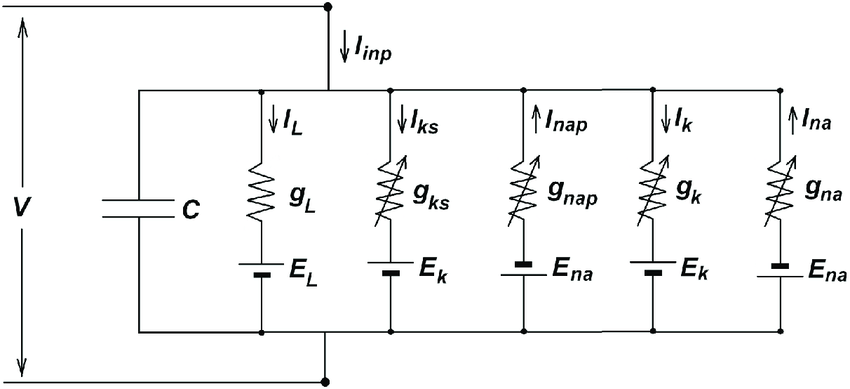
\includegraphics[width=.9\textwidth]{conductanceNet.png}
    \caption{Simplified circuit of the neuron model. (Circuit taken from \citet{electricDiagram})}
    \label{fig:conductance_neuron_circuit}
\end{figure}

This language of currents and potential seems to designate classical circuit theory as a useful tool to model a neuron behavior.
\citet{conductanceModel} were the first to formulate a model of the neuronal behavior using a parallel network of dynamic conductances. 
Those conductances change based on the membrane voltage of the neuron at different rates mimicking the opening and closing of the channels. 
A good representation of this model is seen in \cref{fig:conductance_neuron_circuit}. 
On this diagram, it can be seen that some ionic current discharge the capacity that represent the membrane while other charge it. 
Those charging current effectively act as positive feedback loops. 
As seen in the previous section, those are necessary for the excitable behavior of a neuron.

Using circuit theory, this model can be written more formally using ordinary differential equation. 
\Crefrange{eq:hodgkinstart}{eq:hodgkinend} are a very general representation of this model.
In this representation the $i$ subscript denotes the different ionic currents that can be found in \cref{fig:conductance_neuron_circuit}.

\begin{align}
    C\frac{\partial V}{\partial t} =& I_\text{inp} - g_L\left(V-E_L\right) - \sum_i I_i\label{eq:hodgkinstart}\\
    I_i\left(t, V\right) =& g_i\left(t, V\right)\left(V - E_i\right)\\
    g_i\left(t, V\right) =& \bar{g_i}m_i\left(t, V\right)^{p_i} h_i\left(t, V\right)^{q_i}\\
    \frac{\partial m_i\left(t, V\right)}{\partial t} =& \frac{m_{i\infty}\left(V\right) - m_i\left(t, V\right)}{\tau_{mi}\left(V\right)}\\
    \frac{\partial h_i\left(t, V\right)}{\partial t} =& \frac{h_{i\infty}\left(V\right) - h_i\left(t, V\right)}{\tau_{hi}\left(V\right)}\label{eq:hodgkinend}
\end{align}

The $m_\infty$, $h_\infty$, $\tau_m$ and $\tau_h$ terms follow saturation functions.
The saturation of the $\infty$ terms show that the ionic current feedbacks are localized in a certain range of membrane voltage.
This was expected since excitable behavior requires a localized positive feedback.


This model is very general and, when parameters are chosen properly, it is able to generate a whole range of neuronal behaviors seen in biological neurons. 
In this thesis, only spiking and bursting, the two most common behaviors will be used. Those two behaviors can be seen in \cref{fig:behaviours}. 
A spike is a sudden, short and steep increase in the neuron voltage followed by a sharp decrease and return to a resting voltage. 
A burst is the apparition of a packet of spikes.

Classically both behaviors can be tonic of phasic.
A tonic response means that it is sustained, this is what is observed in \cref{fig:behaviours} where the spike and burst repeat.
A phasic response means that it is transient, the behavior is only caused by a change in the input like in \cref{fig:excitability} and will not continue after the initial response.
Often, for a set of parameters, as the input current increases a neuron will first have a phasic response before starting to become tonic.
% Tonic or not tonic bursting and spiking

\begin{figure}[htb]
    \centering
    \inserttikzfig{plots/neuron_behaviour.tikz}
    \caption{Example of spiking and bursting behaviors. Generated using neuron model of \cref{sec:model}.}
    \label{fig:behaviours}
\end{figure}

\section{Neuronal Behavior Metrics}

As seen before neural behaviors exhibit unusual patterns. 
To be able to compare different bursting or spiking specific metrics must be defined.
Here, only the metrics to evaluate the tonic spiking and the tonic bursting will be discussed.

\Cref{fig:burst_metrics} represents values that can be directly inferred from the trance of a tonic bursting neuron. Those values can be defined as
\begin{description}
    \item[Burst length] The average time of a burst event.
    \item[Rest length] The average time of inactivity between two burst events.
    \item[Burst period] The average time between the starts of two burst events.
    \item[Spike period] Inside a burst, the average time between the start of two spike events.
    \item[Number of spikes] The average number of spikes inside a burst event.
\end{description}

\begin{figure}[htb]
    \centering
    \inserttikzfig{diagrams/burst_metrics.tikz}
    \caption{Illustration of the different metrics used to describe bursting. Generated using neuron model of \cref{sec:model}.}
    \label{fig:burst_metrics}
\end{figure}

Aside from the number of spikes, those raw metrics metrics are not suited to this thesis. 
Instead, the following set of metrics derived from the aforementioned values is used.
\begin{description}
    \item[Inter-burst frequency] $\frac{1}{\text{Burst period}}$, the frequency at which burst events occur.
    \item[Intra-burst frequency] $\frac{1}{\text{Spike period}}$, frequency at which spikes occur inside a burst event.
    \item[Duty cycle] $\frac{\text{Burst length}}{\text{Burst period}}$, the portion of time of a period where the neuron is inside a burst event.
    \item[Number of spikes] The average number of spike inside a burst event.
\end{description}
Even though the inter-burst frequency and the intra-burst frequency are just opposites of direct metrics, the realm of frequencies is often better suited to compare with other things.


The tonic spiking does not require so much metrics. 
The only direct metric is measuring the \textbf{Spike period}.
It is enough to compute the \textbf{Spiking frequency} which is the most useful metric to describe a spiking behavior. 
For the same reason as the bursting transforming in frequencies is better for comparison.


% Types

\section{Central Pattern Generators and Rhythms}

To develop the controller, the concept of central pattern generators (CPGs) is very useful since they are linked closely to rhythmic movement. 
And, the oscillation of a pendulum is a naturally rhythmic movement.

From \citet{cpgDef}, \enquote{A central pattern generator (CPG) is an assembly of neurons that possesses the ability to produce a rhythmic activity pattern without \textdel{phasic} sensory feedback information}.

From this, it id clear that CPGs require multiple neurons to work.

Also, it is widely admitted that central pattern generators are frequently found in biological motion systems. 
\citet{cpgMotion, cpgMotion2} highlight that CPGs are abundant in the control of animals motion.
The natural periodic oscillations of CPGs makes them easier to pair with systems that are already periodic

To keep it simple, the connections between neurons inside a CPG result in the activity of one neuron generating currents in the other neuron. 
Those connections can have two types, inhibitory and excitatory. 
An inhibitory connection results in negative current being injected while an excitatory connection creates a positive current.

The most simple and well studied CPG is the half-center oscillator \citep{halfcenter}. 
This specific circuit is composed of two neurons that inhibit each other. 
The system along with simulation can be seen in \ref{fig:halfcenter}.
The currents flow from one neuron to the other only if the injecting neuron is activated.

\begin{figure}[htb]
    \centering
    \inserttikzfig{diagrams/halfcenter.tikz}
    \caption{Example of an half center oscillator. Traces were generated using neuron model of \cref{sec:model}.}
    \label{fig:halfcenter}
\end{figure}

The generation of rhythmic patterns is clear when looking at the traces of the activation of the different neurons. 
Indeed, the activation of neuron 1 and neuron 2 always follow each other.
This temporal shift can be expressed in term of phase by saying that one neuron as a phase of $\frac{1}{2}$ of a period compared to the other.
But, it will no appear in the game.
% Cite marder or other of different CPGs, show graphs of rythms

\section{Embodied Intelligence and CPGs} 

From \citet{embodiedDef} \enquote{Embodied intelligence is the computational approach to the design and understanding of intelligent behavior in embodied and situated agents through the consideration of the strict coupling between the agent and its environment (situatedness), mediated by the constraints of the agent’s own body, perceptual and motor system, and brain (embodiment).}.

This concept is describing the goal of this thesis.
Indeed , the model that is developed later is a prime example of embodied intelligence. 
The controller will process direct sensory input to generate coherent control signals for the motor. Using neuromodulation the strength of the push will be changed according to a desired amplitude.

More broadly, the concept of embodied intelligence is closely related to CPGs. Indeed, CPGs are circuits that are rhythmic without sensory feedback, but using sensory feedback to tune the frequency of the CPG to the external is thought to be inner working of most biological motion controller (citation needed).
This coupling is precisely a low-level embodied intelligence. 

To Simplify embodied intelligence, it can be seen as the coupling of sensing computing and actuating. 
The agent in embodied learning has its sensors, its computing and its actuation in the same body. 


% Define embodied Intelligence and its relationship with CPGs 
